%File: GMM.tex
%Date: Mon Dec 30 22:05:51 2013 +0800
%Author: Yuxin Wu <ppwwyyxxc@gmail.com>

\subsection{GMM-UBM}

\begin{frame}{GMM}
  \textbf{Gaussian Mixture Model}
  is commonly used to model human's acoustic feature.

  \begin{exampleblock}{}
    \[ p(\theta) = \sum_{i=1}^{K}{w_i \mathcal{N}(\mathbf{\mu}_i, \Sigma_i)}\]
  \end{exampleblock}
  \pause

  \begin{columns}
    \begin{column}{0.5\textwidth}
      \begin{center}
        \only<1>{\includegraphics[width=\textwidth]{res/gmm.png}}
        \visible<2>{ 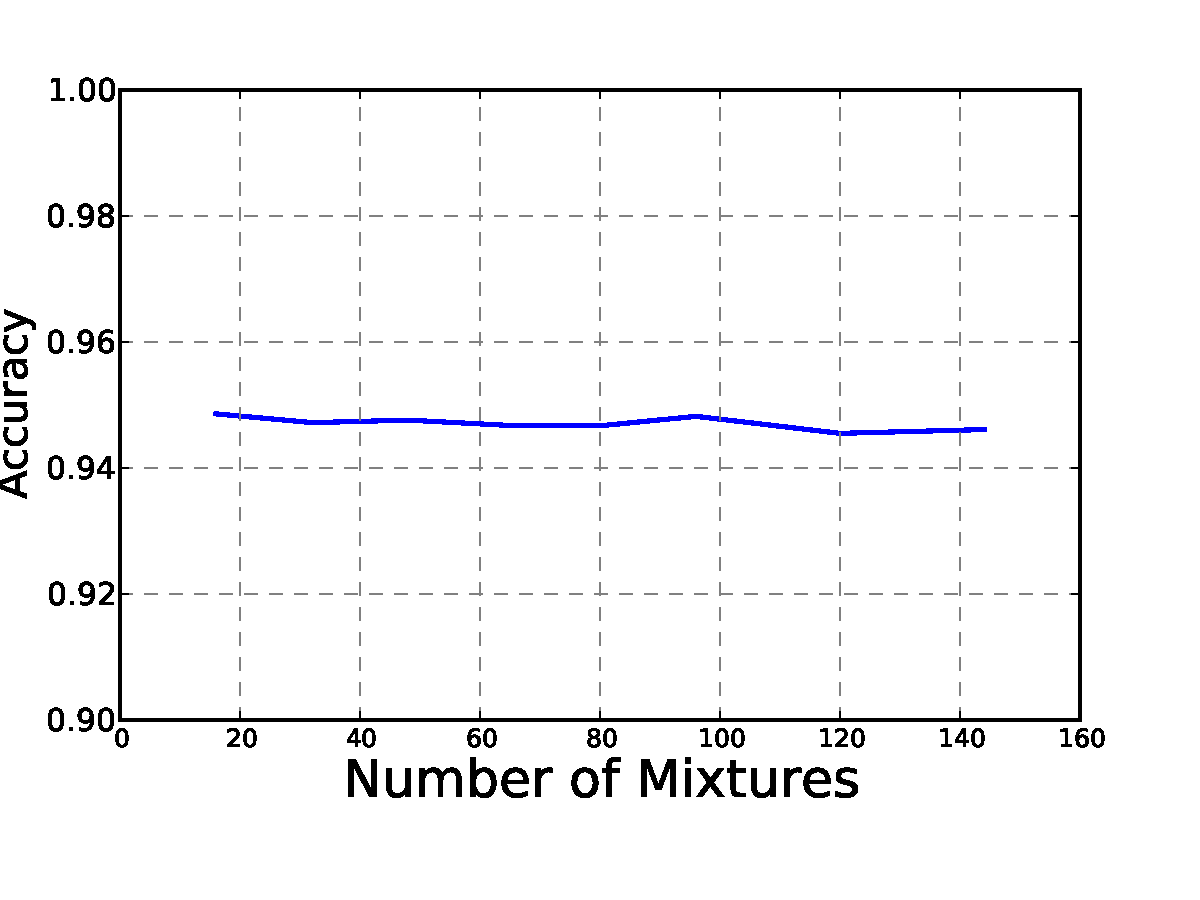
\includegraphics[width=\textwidth]{res/nmixture.pdf} }
      \end{center}
    \end{column}
    \begin{column}{0.3\textwidth}
      We use $ K=32$
    \end{column}
  \end{columns}
\end{frame}

\begin{frame}{Optimized GMM}
  \begin{itemize}
    \item Basic GMM training: random initialize, estimate params with EM.
    \item Improvment: initialize with a parallel KMeans++.
    \item Improvment: parallel training implemented in C++.
    \item Compared to GMM from scikit-learn:
  \end{itemize}

  \begin{columns}
    \begin{column}{0.5\textwidth}
      \begin{center}
        \visible<2>{ 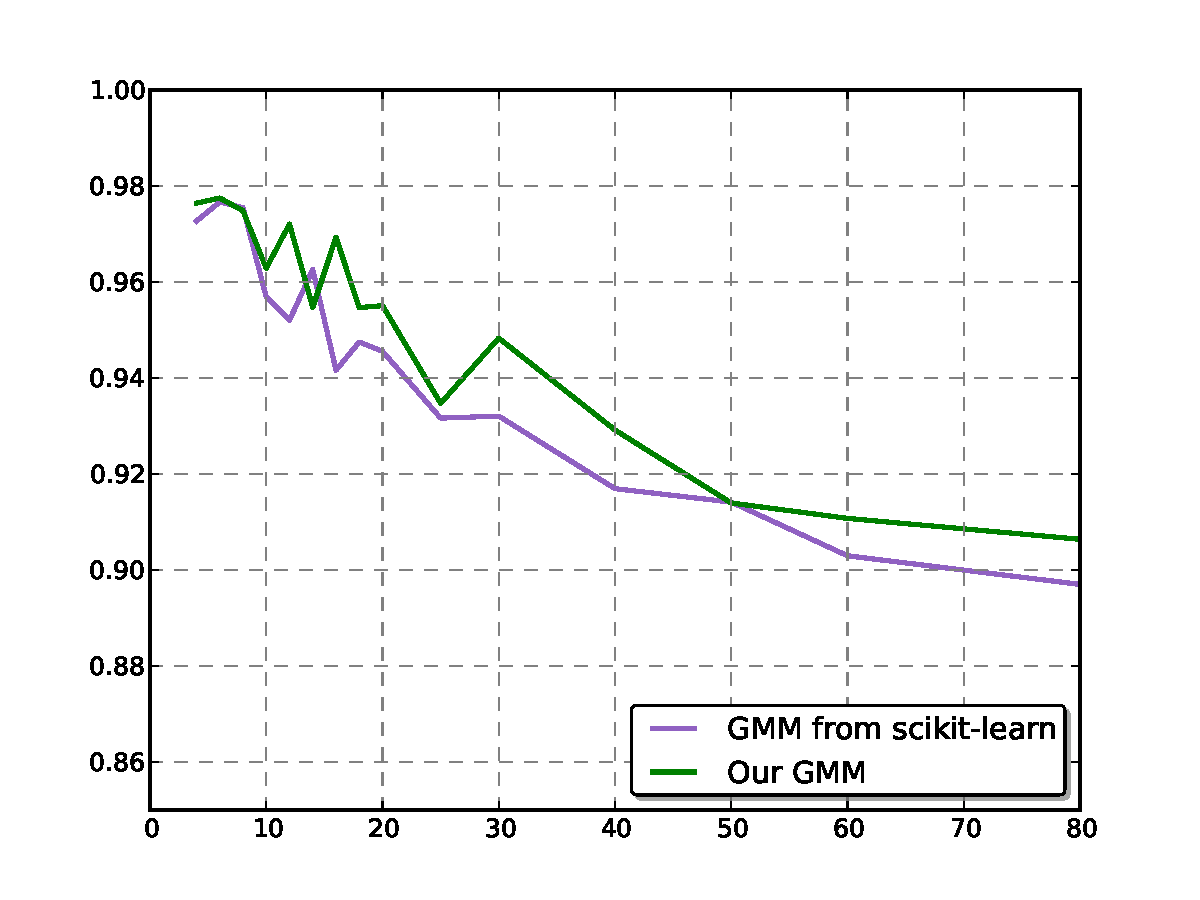
\includegraphics[width=\textwidth]{res/gmm-compare.pdf} }
      \end{center}
      \vspace{0.6em}
    \end{column}
    \begin{column}{0.6\textwidth}
      \visible<2>{ \includegraphics[width=\textwidth]{res/time-comp-small.pdf} }
    \end{column}
  \end{columns}
  \vspace{2em}

  \begin{reference}{4mm}{85mm}
    Arthur, David, Sergei, 2007,
    k-means++: The advantages of careful seeding.

    Scikit-learn: Machine Learning in {P}ython. \url{http://scikit-learn.org}
  \end{reference}
\end{frame}

\begin{frame}{UBM}
  \textbf{Universal Background Model} is a GMM trained on giant datasets.

  UBM can be used to:
  \begin{itemize}
    \item Describe general acoustic feature of human.
    \item Reject the decision of GMM.
    \item Train adaptive GMM.
  \end{itemize}

  \begin{reference}{4mm}{85mm}
    Reynolds, Douglas, et al, 2000,

    Speaker verification using adapted Gaussian mixture models
  \end{reference}
\end{frame}

